\documentclass[letterpaper,12pt]{article}
\usepackage{tabularx} % extra features for tabular environment
\usepackage{amsmath}  % improve math presentation
\usepackage{float}
\usepackage{pdfpages}

\usepackage{graphicx} % takes care of graphic including machinery
\graphicspath{ {./figures/} }
\usepackage[margin=1in,letterpaper]{geometry} % decreases margins
\usepackage{cite} % takes care of citations
\usepackage[final]{hyperref} % adds hyper links inside the generated pdf file
\hypersetup{
	colorlinks=true,       % false: boxed links; true: colored links
	linkcolor=blue,        % color of internal links
	citecolor=blue,        % color of links to bibliography
	filecolor=magenta,     % color of file links
	urlcolor =blue         
}




\begin{document}

\title{Spring 2022 EE214 Experiment 1  \protect\\ Diodes and Rectifiers}
\author{Ahmet Akman 2442366 \protect\\ Yusuf Toprak Yıldıran 2444149}
\date{\today}
\maketitle
\tableofcontents
%\begin{abstract}
%abstract
%\end{abstract}
\section{Introduction}
In this document the actions corresponding requirements defined in the Experiment Manual are  represented.

\section{Experimental Results and Discussion}

\subsection{Step 1}

\begin{figure}[H]
\centering
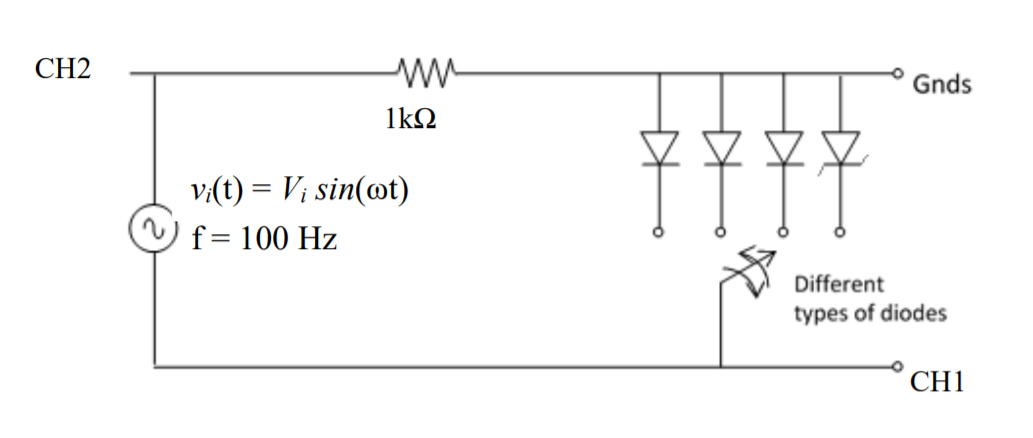
\includegraphics[width=1\textwidth]{1_1.png}
\caption{Circuit schematic for the step 1}
\end{figure} 

\subsubsection{a)}
\subsubsection{b)}


We can call separation of lines in i-v graph as hysteresis effect. When we increase frequency to 10kHz, we observed hysteresis effect on the i-v characteristics of diode on the DSO screen. Since our diode can not change its state as fast as our high frequency voltage source supply, we observe this effect. To solve this problem and to be able to use diodes at high frequencies, there are "high speed" or "switching" diodes. These diodes can be used in high frequencies without observing hysteresis effect.

\subsection{Step 2}

\begin{figure}[H]
    \centering
    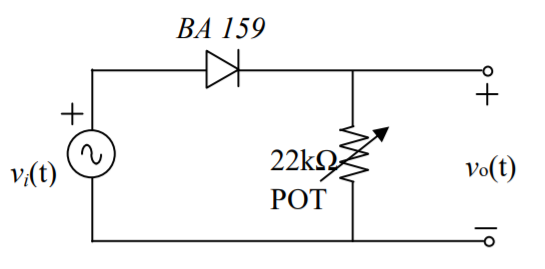
\includegraphics[width=1\textwidth]{2_1.png}
    \caption{Circuit schematic for the step 2}
\end{figure} 
For this part, we set the half-wave rectifier circuit given in Figure X and adjusted 
\(
v_i(t)  = 2sin(2000 \pi t) V 
\)


\subsubsection{a)}
After setting POT to \(1k\Omega\) , we obtain output and input voltage waveforms on the graph indicaded in Figure X.


If we look at the graph carefully, we can realized that output voltage is slightly lower than input voltage since diode consumes energy. Then we measured the \(DC_{rms} \) of output value as 730mV using cursors of DSO. Output voltage waveform on the DSO screen is like same with the input waveform in positive cycles but zero when input is in the negative cycle.  


\subsubsection{b)}


\subsection{Step 3}

In this third step, we set up the diode clamper circuit given in Figure X using the diode 1N4001 and set the voltage \(v_i(t) = 10sin(200\pi t) V\). Then plotted the input and output voltage waveforms on the graph given in Figure X.

From above graph we can derive that output waveform is just shifted form of input waveform to below zero. Since diode prevent capacitor from discharged, in order peak value of output to be clamped above zero diode should go into negative bias.

\begin{figure}[H]
    \centering
    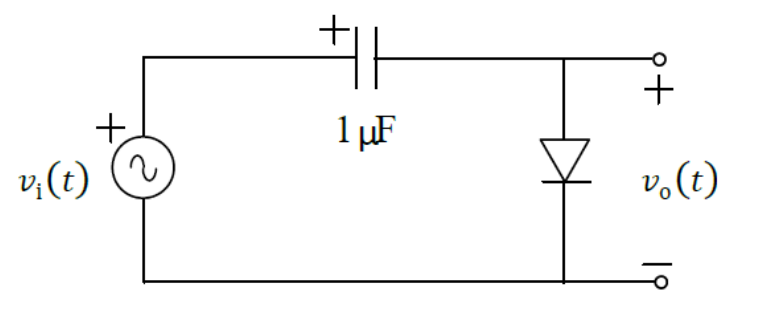
\includegraphics[width=1\textwidth]{3_1.png}
    \caption{Circuit schematic for the step 3}
\end{figure} 
    
    

\subsection{Step 4}

\begin{figure}[H]
    \centering
    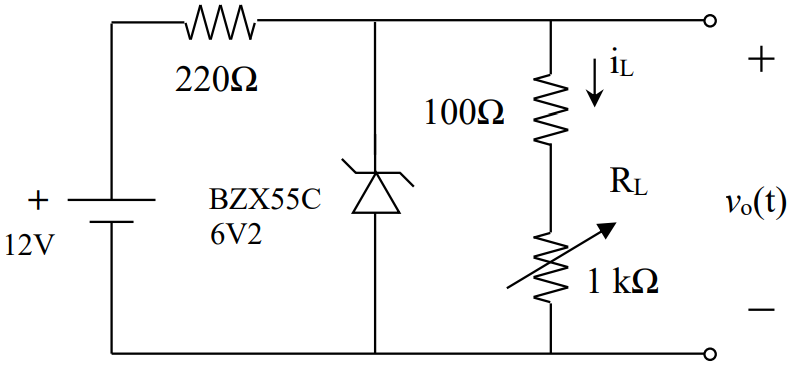
\includegraphics[width=1\textwidth]{4_1.png}
    \caption{Circuit schematic for the step 4}
\end{figure} 
    
    
\section{Conclusion}
asdfd
\section*{Appendix A}
\begin{itemize}
    \item PreLab Preprataion 6 hours
    \item Experimental Work 2  hours
    \item Report Wrining 6 hours
\end{itemize}

\end{document}

%%%%%%%%%%%%%%%%%%%%%%   EXAMPLE TABLE   %%%%%%%%%%%%%%%%%%%%%%%%%%%%%%%%
\begin{table}[H]
\begin{center}
    \caption{Resistance reading by color code convention.}
    \vspace{2mm}
    \begin{tabular}{||c | c | c||} 
        \hline
        Color Order & Value & Tolerance \\ [0.5ex] 
        \hline\hline
        Brown / Black / Red / Gold & 1k\( \Omega \) & \( \% \) 5  \\ 
        \hline
        Yellow / Violet / Red / Gold & 4.7k\( \Omega \) & \( \% \) 5   \\
        \hline
        Brown / Grey / Orange / Gold & 18k\( \Omega \) & \( \% \) 5  \\ [1ex] 
        \hline
    \end{tabular}
\end{center}
\end{table}


%%%%%%%%%%%%%%%%%%%%%%   EXAMPLE IMAGE   %%%%%%%%%%%%%%%%%%%%%%%%%%%%%%%%
\begin{figure}[H]
\centering
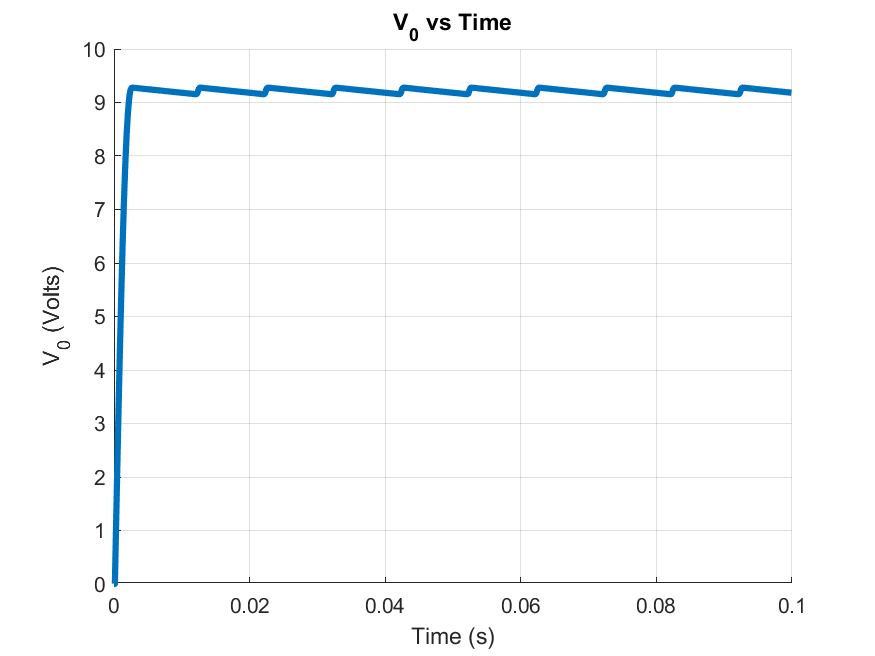
\includegraphics[width=1\textwidth]{5.png}
\caption{Circuit schematic for the step 5}
\end{figure} 

%%%%%%%%%%%%%%%%%%%%%%   EXAMPLE IMAGE FROM PDF   %%%%%%%%%%%%%%%%%%%%%%%%%%%%%%%%
\begin{figure}[H] \centering{
	\includegraphics[scale=0.25]{2a_plot.pdf}}
	\caption{Experiment 2}
\end{figure}
	